\documentclass{article}
\usepackage[utf8]{inputenc}
\usepackage{amsfonts}
\usepackage{amsmath, bm}
\usepackage[a4paper, margin=1in]{geometry}
\usepackage{fancyhdr}
\usepackage{mathptmx}
\usepackage{multicol}
\usepackage{lipsum}
\usepackage{setspace}
\usepackage{graphicx}
\usepackage{float}
\usepackage{algorithm}
\usepackage{algpseudocode}
\usepackage{makecell}
\usepackage{adjustbox}
\usepackage{tabularray}
\usepackage{xcolor}

\usepackage[font=footnotesize]{caption}


\onehalfspacing

\title{
\noindent\vrule height 2.5pt width \textwidth
\begin{center}
    \bfseries AutoCat - Auto Embedding for Categorical Features
\end{center}
\noindent\vrule height 2.5pt width \textwidth
}
\author{\bfseries Rotem Gazit \thanks{ID: 318446697}}
\date{}


\begin{document}

\maketitle


\begin{abstract}
\bfseries
Although categorical features appear everywhere, they create enormous problems to existing learning methods. The ambiguity they create regarding their numerical representation -- whether they are nominal or ordinal, creates a great challenge for every learning algorithm to fully utilize them, and demand the data scientists to manually embed them properly. While common practices like One-Hot Encoding avoid the question of ordinality, they demand much more complex algorithms. Here, AutoCat is introduced -- an automatic embedding solution for categorical features. Using the target variable, AutoCat automatically detects ordinal features and sorts them in the right way, and applies the One-Hot encoding only on nominal features, thus allowing for more efficient learning. AutoCat outperformed naive embedding approaches in both regression and classification tasks, without changing the model complexity.
\end{abstract}

% \begin{multicols}{2}
\section{Introduction}
In almost every tabular dataset, One can find some categorical or ordinal features. These features capture fundamental aspects in the examined domain - they might represent someone’s gender or level of education, the color of a product, or the car’s manufacturer. Although these features might stand at the core of the task we intend to perform, most common models – including regression-based models, tree-based models, or neural networks – are not natively designed to benefit from them, thus some kind of data preparation process must be performed beforehand. This data preparation process, also known as feature engineering, is usually done manually.

A categorical feature consists of two or more categories, which may or may not be correlated to the dependent variable we intend to predict. \textbf{Nominal Categorical Features} are defined as a list of labels without any immediate way of sorting them, e.g., gender or car manufacturer. Also, \textbf{Ordinal Categorical Features} are defined as features with some kind of natural way to sort them, e.g., education level. Note that in many cases these features are not numerical, thus deciding whether a feature is ordinal (and consequently finding the right ordering) is not trivial.

When done correctly, embedding these categorical features can significantly boost the performance of a model. For example, a tree-based model would benefit from the ordinal sorting of a feature as it can achieve the same performance with shallower trees. 
Common representation of these features are the One-Hot encoding, where each category is modelled as a different binary feature, and Label-Encoding, where we assign an integer to replace each label.

Here, I introduce AutoCat -- a python library designed to automatically detect and embed categorical features. AutoCat uses the target variable of the training set in order to surmise if the feature is nominal or ordinal, and if it is indeed the latter -- sort it in the right order. AutoCat replaces the manual feature engineering process needed when handling categorical features, and is able to significantly boost the performance of the applied algorithm.

\section{Related Work}
Many previous works have reviewed the domain of categorical data analysis, both from the statistical point of view, and for machine-learning algorithms \cite{agresti2018introduction, Stevens1946}. Ordinal scales defer from nominal by having a ranking, but they both do not have scaling (for interval or ratio). That is, although the ordinal categories "Small", "Medium" and "Large" have clear ranking ("Small" $<$ "Medium" $<$ "Large"), there is no way to quantify how big is the "gap" between each consecutive pair.

The One-Hot Encoding converts a set of categories $C = \{c_1, \dots, c_k\}$ into sparse vectors $\{0, 1\}^k$. This encoding detaches any kind of ordinal sorting the categories might have had, and regards each possible category as a new binary feature.
Recent works reviewed the usage of different embedding approaches for machine learning \cite{Potdar2017}, suggesting that the One-Hot Encoding performs better than any other embedding technique, but comes with higher cost in model complexity. 
Other works reduce the number of dimensions used in One-Hot Encoding for the target labels, instead of features, using training samples \cite{Rodrguez2018}.

Originaly, categorical data analysis laid the foundations for measuring the association between nominal and ordinal features. Many association measures are based upon the $\chi ^2$ statistic: Cramér's V measures the association between two nominal variables \cite{cramer1999mathematical}, The $M^2$ statistic measures the association between two ordinal features \cite{agresti2007an}. Measuring the association between ordinal and continuous variables can be done using other common association metrics, such as Pearson or Spearman correlation coefficients. 

\section{AutoCat}
The main problem in utilizing categorical features lays in the fact that there is no immediate relation between the categories. As most learning algorithms refer to each feature as numerical, randomly assigning a numerical representation for each category may have catastrophic effect over the performance of the algorithm, or to heavily affect its complexity (Figure \ref{figure:fig1}). Moreover, in some cases, the categories have no ordinal meaning, so enforcing some order over them may result in a big dropout in performance between training and testing. The One-Hot Encoding became popular as it removes the need for picking the right order of categories, but demand more complex models, as the number of features is effectively larger. 

Here, I suggest mitigating this problem by looking for the optimal ordinal representation of categories, or to use the One-Hot Encoding if such ordering could not be found. First, I remove smaller categories and bin them into several default classes, in order to reduce the number of categories needed to explore. Next, I greedily sort the categories using the target variable as a guild line for detecting their inner structure. Finally, the resulting sorted categorical representation is evaluated and neglected if the inner structure does not seem to be ordinal.

\begin{figure*}
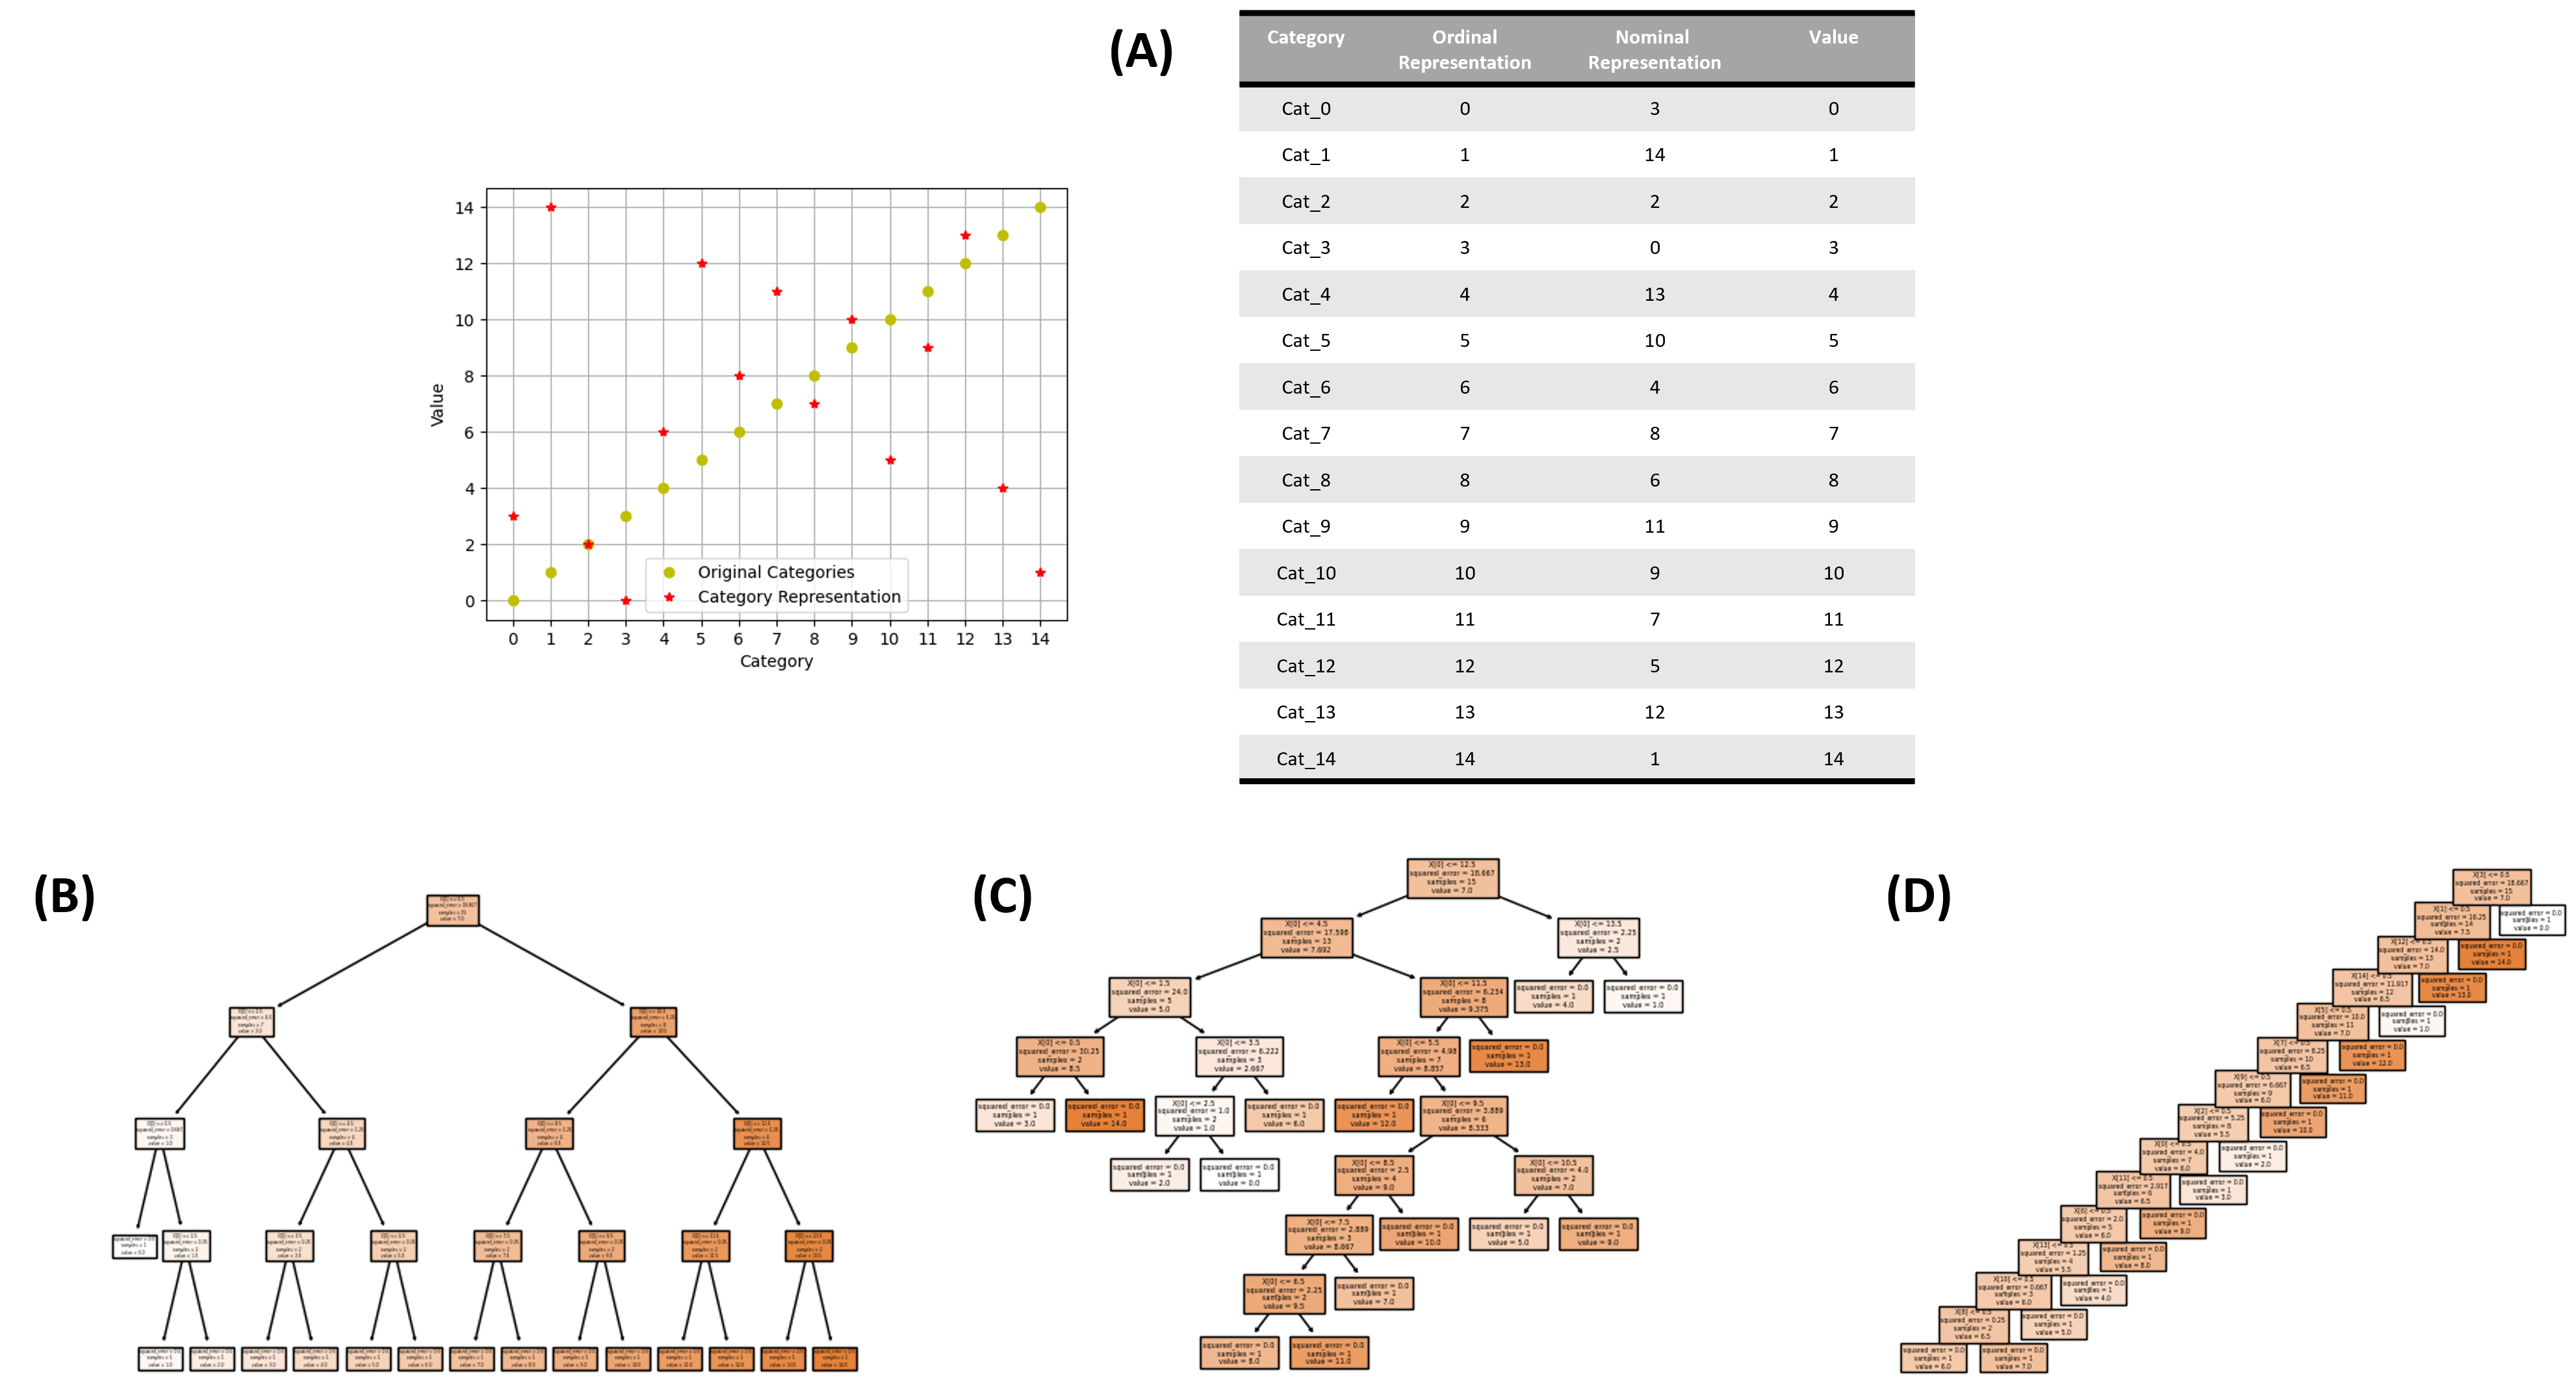
\includegraphics[width=\textwidth]{imgs/figure1}

\caption{\label{figure:fig1}
\textbf{The effect of various categorical representations on the efficiency of a decision tree regressor.} \\
Darker colors in the decision trees \textbf{(B-D)} represent higher predicted values.\\
\textbf{(A)} A dataset with 15 categories ("category" column), which are linearly correlated to the target variable ("value" column). The "nominal representation" column randomly shuffles the labels of each category. $R(\text{Ordinal Repr.}, \text{Value})=1, R(\text{Nominal Repr.}, \text{Value})=0.032$ \\
\textbf{(B)} A decision tree regressor fitted over the ordinal representation and the target value. The tree is relatively shallow and well-balanced, (depth = 4), which makes this representation the most efficient in terms of model complexity. \\
\textbf{(C)} A decision tree regressor fitted over the nominal representation and the target value. Unlike \textbf{(B)}, the tree is much deeper and unbalanced (depth = 8). When the decision tree regarded the nominal representation as numerical, it demanded a more complex model for achieving the same results as (B) \\
\textbf{(D)} A decision tree regressor fitted over the One-Hot encoding and the target value. Here we find the deepest tree (depth = 14). \\
}
\end{figure*}

\subsection{Dropping Rare Categories}
Too many categories, where a big portion of them is rare -- meaning, that there is only a very small number of samples in the dataset to represent them, creates an unnecessary challenge for many learning algorithms. Unlike numerical features, where One would expect the algorithm to generalize from nearby samples, categories bear no scale or immediate ordering for such generalization to emerge. Hence, a common technique for handling categorical variables is to merge several smaller categories into bigger ones. 

Let $X=\{x_i \in C\}_{i=1}^N$ be a feature of categories $C=\{c_1,\dots,c_k\}$. A category $c\in C$ is called Unpopular if its fraction of samples is less than a given $\epsilon$: 
$$\frac1N \sum_{i=1}^{N}\mathbb{I}_{[x_i = c]} < \epsilon$$

Let $C_\epsilon \subseteq C$ be the unpopular categories, $C_\epsilon = \{c \in C\ \vert \ \frac1N \sum_{i=1}^{N}\mathbb{I}_{[x_i = c]} < \epsilon \}$. The simplest solution is to replace them all with a dummy category $C^*$. 

Furthermore, if the target variable is continuous, i.e., $Y = \{y_i \in \mathbb{R}\}_{i=1}^N$, One can replace $C_\epsilon$ with several dummy categories in order to maintain their various impact over the target. Let $Y_c = \{y_i\ \vert\ x_i = c\}$ be the targets for the samples in category $c\in C$. By binning $C_\epsilon$ using their mean target values $\bar{Y}_c$ into $t$ subsets, One can replace them with $\{C_i^*\}_{i=1}^t$ dummy categories.

Overall, the resulting set of categories is now smaller, and most importantly -- stabler, as it is less sensitive to training set sampling (which might have missed the rarest of categories).

\subsection{Embedding for Regression}
Most of the models designed for regression problems, implicitly or explicitly utilize from features with higher correlation to the target variable. For example, Linear Regression tries to directly quantify the linear correlation between features and target. Decision-Tree based methods benefit from a linearly-correlated feature, as every "cut" it makes affects the predicted value more dramatically. Therefore, if the categorical feature can be mapped in a way that maximizes the correlation to the target variable, it may significantly improve the model's performance without introducing additional complexity in training.

Let $X=\{x_i \in C\}_{i=1}^N$ be a feature of categories $C=\{c_1,\dots,c_k\}$, and let $Y=\{y_i\}_{i=1}^N$ be the target. Also, let $\rho$ be a correlation coefficient metric. 
A one-to-one mapping of categories $f: C\to\{1,\dots,k\}$ is considered optimal, according to  the target variable and the given $\rho$, if $\rho(f(X), Y)$ is maximal.
For instance, if $\rho = R$ the Pearson Correlation Coefficient, such optimal mapping would make $f(X)$ as linearly correlated as possible to the target $Y$. In other words, if we regard $f(X$) as a numerical feature, it will be as correlated to $Y$ as it can get.

Since there are $k!$ possible mappings to examine, a direct search for such optimal $f$ might be computationally expansive. Instead, a more greedy approach could be taken. Let $X_j = \{\mathbb{I}_{[x_i = c_j]}\}_{i=1}^N$ the One-Hot encoding of feature $X$ according to category $c_j$, and let $\rho_j = \rho(X_j,Y)$. 
The selected mapping $f$ is defined by sorting $\{\rho_j\}$ in increasing order, 
$f(c_i) \leq f(c_j) \iff \rho_i \leq \rho_j$. Again, when considering the Pearson Correlation Coefficient, the resulting $f$ sorts the categories from the most negatively-correlated to the target variable to the most positively-correlated one.

However, if the mapping $f$ only has a small correlation to the target variable, i.e. $\rho(f(X), Y) < \epsilon$, 
It might suggest that $X$ is actually a nominal feature, meaning that there is no "right"  sorting, and instead the feature is embedded using the One-Hot encoder.

\subsection{Embedding for Classification}
Classification problems use a categorical target variable, $Y=\{y_i \in \{1, \dots, L\}\}$, and therefore generalizing the same method used for regression problems is not possible. Although there are measures of correlation between a categorical feature $X=\{x_i \in C\}_{i=1}^N$ and $Y$, such as Cramér's V \cite{cramer1999mathematical}, which are based upon the $\chi^2$ test, they are not helpful in finding the ordinal sorting of categories as they bear no directional meaning -- they only quantify the correlation in the range $[0,1]$ (0 means no correlation, 1 means full correlation). I found these correlation measures to be unhelpful for finding the right ordinal meaning (Figure \ref{figure:fig2}).

Instead, the categories are sorted according to similarities in their effect over target classes. Two categories are considered "similar" if the probability of finding the different classes of the target variable in them is close. Let  $X=\{x_i \in C\}_{i=1}^N$ a categorical feature of categories $C=\{c_1,\dots,c_k\}$, and let $Y=\{y_i \in \{1, \dots, L\}\}$ the target of $L$ classes. For each category $c_i \in C$, let 
\begin{align*}
\omega_{i,j} & = \sum_{i=1}^k \sum_{j=1}^L \mathbb{I}_{[x_i = c_i]} \cdot \mathbb{I}_{[y_i = j]} \\
\bar{\omega}_i & = \frac{1}{\sum_{j=1}^L \omega_{i,j}} (\omega_{i,1}, \dots, \omega_{i, L}) \\
\omega &= \{\bar{\omega}_i \}_{i=1}^k
\end{align*}

$\bar{\omega}_i$ can be seen as a representation in $[0,1]^L$ of each category in $C$, and the goal is to sort $C$ is such a way that nearby $\bar{\omega}_i, \bar{\omega}_j$ should have nearby ordinal values. Analogically, it is equivalent to finding the minimal path for travelling through $\omega$, which can be found by searching for the minimal spanning tree in $\omega \times \omega$.

Let $G=(\omega, \omega \times \omega, \|\cdot\|_2)$ the full graph of $k$ nodes. Let $T$ be the minimal spanning tree of $G$, and let $\omega_{I_1} \to \omega_{I_2} \to \dots \to \omega_{I_k}$ be the depth-first path from one of its two roots. $f(c_i) = I_i$ is the resulting one-to-one mapping of categories in $C$.

$f$ captures a sort of categories with the most graduate effect over the target classes -- there are minimal overall changes in the ratio of each class between two nearby categories. Figure \ref{figure:fig2} illustrates how this method has successfully found the right order of categories.

Similarly to regression, in order to distinct between ordinal and nominal variables, if $\varphi(f(X), Y) = \varphi(X, Y) < \epsilon$, where $\varphi$ is Cramér's V correlation coefficient, the One-Hot encoding is used instead of the resulting $f$.

\begin{figure*}
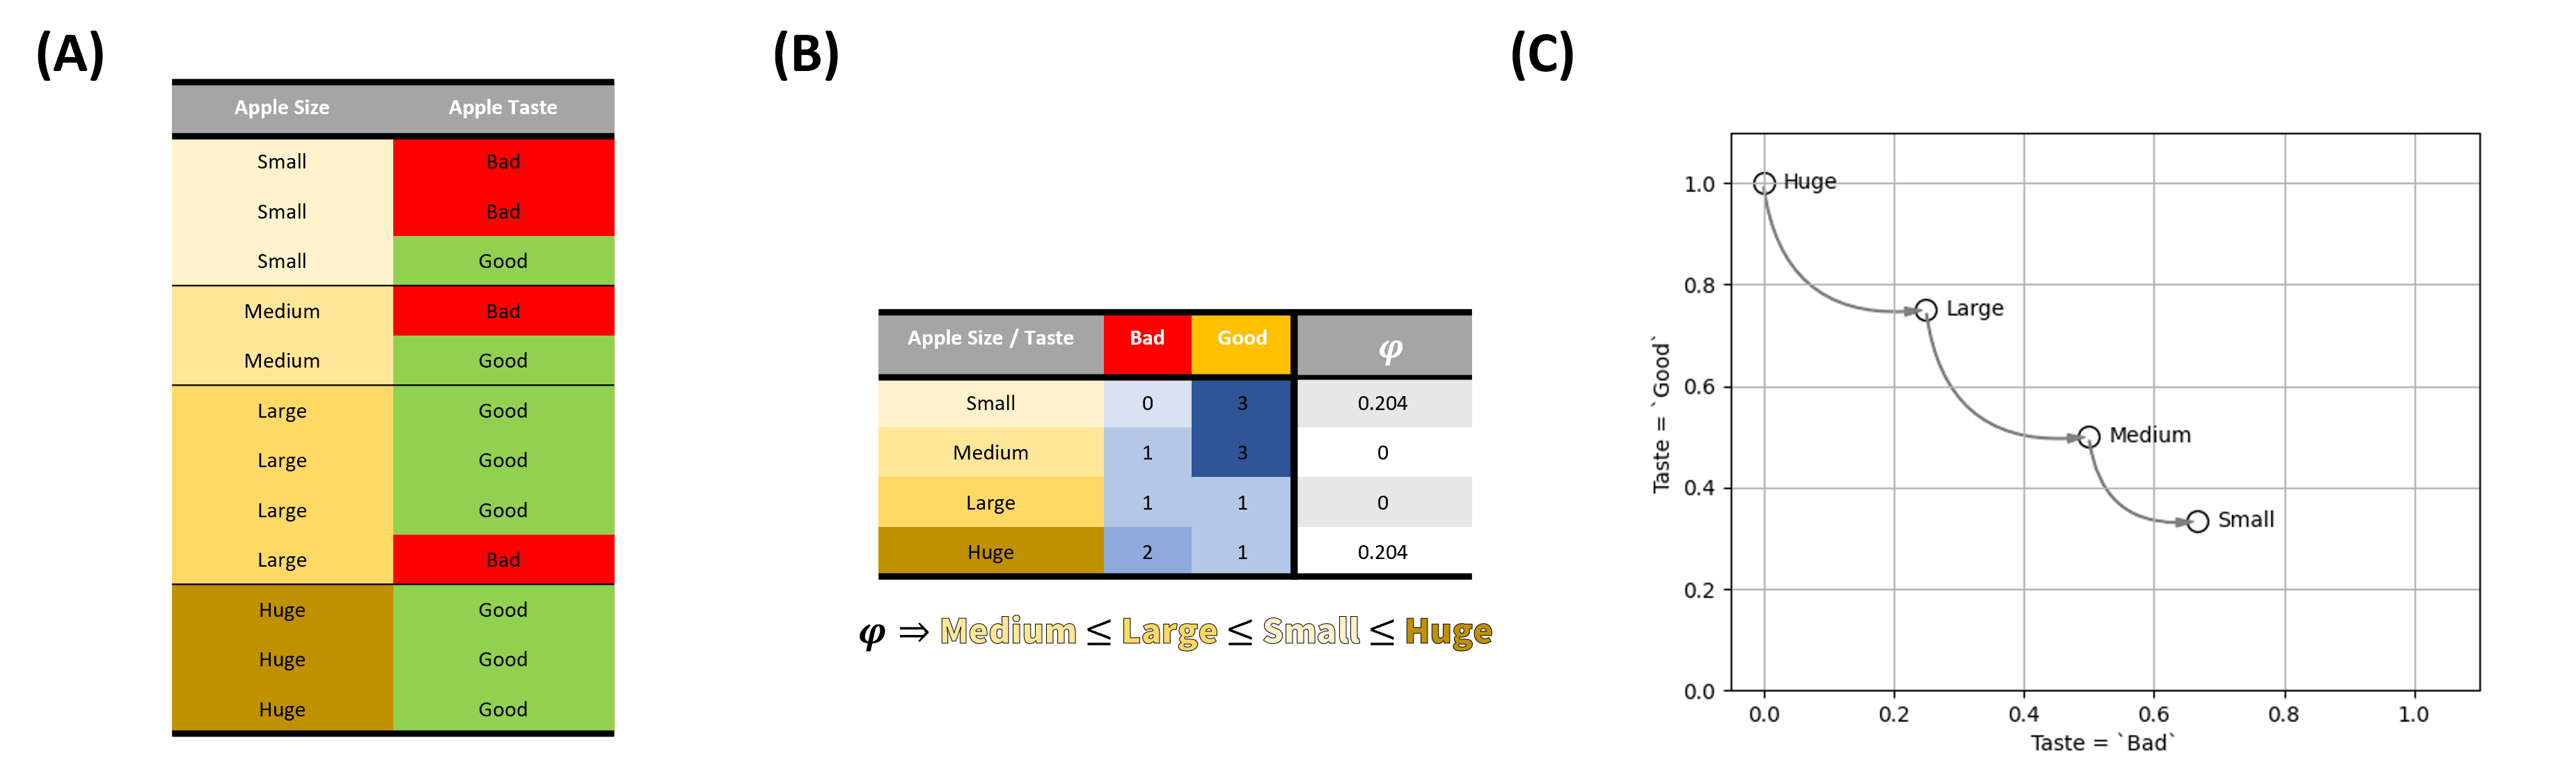
\includegraphics[width=\textwidth]{imgs/figure2}

\caption{\label{figure:fig2}
\textbf{Finding the ordinal sorting for classification models.} \\
\textbf{(A)} A dataset with 4 categories and two target classes. \\
\textbf{(B)} The cross tabulation of (A). Let $\varphi_{c_i} = \text{Cramér'sV}(\mathbb{I}_{[X = c_i]}, Y)$ the Cramér's V correlation between the one-hot representation of each category. This measure cannot help in finding the right order of categories. \\
\textbf{(C)} The values of $\omega_{c_i}$ and the order found using the minimal spanning tree. $\omega_{c_i}$ captures the ratio of each class in the samples of a single category. By regarding the set of points $\omega = \{\omega_{c_i}\}_{c_i \in C}$ as a full graph, and finding the minimal spanning tree with regard to the distance between these points, the right sort of categories was detected (gray arrows).
}
\end{figure*}

\section{Experimental Results}
\label{section:results}

I applied the AutoCat embedding over several real and synthetic datasets, and measured its impact over the performance of multiple learning algorithms, when compared to the naive ordinal embedding of each categorical feature -- that is, assigning a random integer to each category.

I used 2 real datasets and 3 synthetic dataset generators to test the new embedding. For regression, I used the "Car Price in Poland" dataset taken from Kaggle \cite{carPricesPoland}, as well as a linear regression generator and the Friedman dataset generator \cite{Friedman1991}. For classification, I used the "Australian Weather" dataset taken from Kaggle \cite{rainInAustralia}, and a classification dataset generator \cite{scikit-learn}.

For each of the synthetic datasets, I randomly selected a subset of the numerical features and then either binned them into categories or just randomly assigning categories to them, and then shuffled their labels. This created random categories with either ordinal or nominal meaning, but without exposing the underlining embedding.

For each categorical feature $X$ with $C$ categories, I find and convert the unpopular categories, i.e., categories that are only observed in less than $\epsilon = 0.5\%$ of the records, into a dummy category $C^*$ (or, as described in the previous section, into multiple ($t=3$) dummy variables). Next, I find the mapping $f: C\to \{1,\dots, |C|\}$ using AutoCat and apply $\tilde{X} = f(X)$.

In order to evaluate the performance of AutoCat, I compare the performance of several models -- Tree based (Random Forest \cite{Ho95} and XGBoost \cite{Chen:2016:XST:2939672.2939785}) and regression based (Linear regression or Logistic Regression). I find AutoCat to outperform conventional methods in almost all the scenarios examined. Each dataset is divided into a random train and validation set ($20\%$ validation). AutoCat is fitted only on the training set, and deployed on the validation set. Each experiment was run 20 times, and p values were calculated using one-sided t-test. 

Overall, AutoCat increased the $R^2$ in $25\%$ on average, decreased the mean absolute error (MAE) in $16\%$ on average (for regression problems), and increased the F1 score in $3.2\%$ on average (for classification problems).

% \begin{table}
% \begin{adjustbox}{width=\columnwidth,center}
\begingroup
\footnotesize
\begin{longtblr}[
  caption = {AutoCat Performance},
  label = {tab:test},
]{
  colspec = {|X[0.7]X[0.3]XXXX[0.7]|},
  rowhead = 1,
  hlines,
  row{even} = {gray9},
  row{1} = {olive9},
} 
 \textbf{Dataset} &
 \textbf{Type} & 
 \textbf{Model} & 
 \textbf{Random Ordinal} & 
 \textbf{AutoCat} &
 \textbf{$\mathbb{P}(\frac{\text{AutoCat}}{\text{Random}} = 1)$}
 \\
 Car Prices & R &
 \makecell[l]{Random Forest Regressor \\ max depth = 10 } 
    & \makecell[l]{ $R^2 = 0.915 \pm 0.004$ \\ $\text{MAE} = 0.194 \pm 0.004$ }
    & \makecell[l]{ $\bm{ R^2 = 0.929 \pm 0.005 }$ \\ $\bm{ \text{MAE} = 0.174 \pm 0.004 }$ }
    & \makecell[l]{ $p_{R^2} < 0.001$ \\ $p_{\text{MAE}} < 0.001$ }
    \\
 Car Prices & R &
  \makecell[l]{ Linear Regression } 
    & \makecell[l]{ $R^2 = 0.83 \pm 0.012$ \\ $ \text{MAE} = 0.274 \pm 0.005 $}
    & \makecell[l]{ $\bm{ R^2 = 0.886 \pm 0.009} $ \\ $\bm{ \text{MAE} = 0.225 \pm 0.005 }$}
    & \makecell[l]{ $p_{R^2} < 0.001$ \\ $p_{\text{MAE}} < 0.001$ }
    \\
  Car Prices & R &
  \makecell[l]{XGBoost Regressor \\ max depth = 5 } 
    & \makecell[l]{ $R^2 = 0.918 \pm 0.004$ \\ $ \text{MAE} = 0.194 \pm 0.004 $}
    & \makecell[l]{ $\bm{ R^2 = 0.921 \pm 0.005 }$ \\ $\bm{ \text{MAE} = 0.188 \pm 0.006 }$}
    & \makecell[l]{ $p_{R^2} = 0.006$ \\ $ p_{\text{MAE}} < 0.001 $}
    \\
 Friedman & R &
 \makecell[l]{Random Forest Regressor \\ max depth = 10 }
  & \makecell[l]{ $R^2 = 0.625 \pm 0.216$ \\ $ \text{MAE} = 2.342 \pm 0.669 $}
  & \makecell[l]{ $\bm{R^2 = 0.717 \pm 0.264 }$ \\ $\bm{ \text{MAE} = 1.883 \pm 0.957 }$}
  & \makecell[l]{ $p_{R^2} = 0.001$ \\ $ p_{\text{MAE}} < 0.001 $}
    \\
 Friedman & R &
  \makecell[l]{ Linear Regression } 
  & \makecell[l]{ $R^2 = 0.211 \pm 0.158$ \\ $ \text{MAE} = 3.51 \pm 0.384 $}
  & \makecell[l]{ $\bm{ R^2 = 0.635 \pm 0.193 }$ \\ $\bm{ \text{MAE} = 2.297 \pm 0.632 }$}
  & \makecell[l]{ $p_{R^2} = 0.005$ \\ $ p_{\text{MAE}} < 0.001 $}
    \\
  Friedman & R &
  \makecell[l]{XGBoost Regressor \\ max depth = 5 } 
  & \makecell[l]{ $R^2 = 0.746 \pm 0.182$ \\ $ \text{MAE} = 1.899 \pm 0.759 $}
  & \makecell[l]{ $\bm{ R^2 = 0.772 \pm 0.201 }$ \\ $\bm{ \text{MAE} = 1.709 \pm 0.904 }$}
  & \makecell[l]{ $p_{R^2} < 0.001$ \\ $ p_{\text{MAE}} < 0.001 $}
    \\
 Synth. Linear & R &
 \makecell[l]{Random Forest Regressor \\ max depth = 10 }
  &\makecell[l]{ $R^2 = 0.571 \pm 0.162$ \\ $ \text{MAE} = 81.073 \pm 24.026 $}
  &\makecell[l]{ $\bm{R^2 = 0.64 \pm 0.185 }$ \\ $\bm{ \text{MAE} = 73.446 \pm 26.364 }$}
  &\makecell[l]{ $p_{R^2} < 0.001 $ \\ $ p_{\text{MAE}} < 0.001 $}
    \\
 Synth. Linear & R &
  \makecell[l]{ Linear Regression } 
  &\makecell[l]{ $R^2 = 0.386 \pm 0.171$ \\ $ \text{MAE} = 90.472 \pm 28.474 $}
  &\makecell[l]{ $\bm{R^2 = 0.745 \pm 0.114}$ \\ $ \bm{\text{MAE} = 55.909 \pm 20.532 }$}
  &\makecell[l]{ $p_{R^2} < 0.001 $ \\ $ p_{\text{MAE}} < 0.001 $}
    \\
  Synth. Linear & R &
  \makecell[l]{XGBoost Regressor \\ max depth = 5 } 
  &\makecell[l]{ $R^2 = 0.716 \pm 0.133$ \\ $ \text{MAE} = 72.063 \pm 15.97 $}
  &\makecell[l]{ $\bm{R^2 = 0.722 \pm 0.135}$ \\ $ \bm{\text{MAE} = 70.544 \pm 16.204 }$}
  &\makecell[l]{ $p_{R^2} = 0.027$ \\ $ p_{\text{MAE}} = 0.002 $}
    \\
 Synth. Class. & C &
 \makecell[l]{Random Forest Classifier \\ max depth = 20 }
  &\makecell[l]{ $R^2 = 0.872 \pm 0.033$ \\ $ F_1 = 0.871 \pm 0.033 $}
  &\makecell[l]{ $\bm{R^2 = 0.89 \pm 0.041}$ \\ $\bm{ F_1 = 0.89 \pm 0.041 }$}
  &\makecell[l]{ $p_{R^2} < 0.001$ \\ $ p_{F_1} < 0.001 $}
    \\
 Synth. Class. & C &
  \makecell[l]{ Logistic Regression } 
  &\makecell[l]{ $R^2 = 0.692 \pm 0.061$ \\ $ F_1 = 0.689 \pm 0.064 $}
  &\makecell[l]{ $\bm{R^2 = 0.795 \pm 0.045}$ \\ $\bm{ F_1 = 0.795 \pm 0.045 }$}
  &\makecell[l]{ $p_{R^2} < 0.001$ \\ $ p_{F_1} < 0.001 $}
    \\
  Synth. Class. & C &
  \makecell[l]{XGBoost Classifier \\ max depth = 20 } 
  &\makecell[l]{ $R^2 = 0.881 \pm 0.036$ \\ $ F_1 = 0.882 \pm 0.035 $}
  &\makecell[l]{ $\bm{R^2 = 0.897 \pm 0.034}$ \\ $ \bm{F_1 = 0.897 \pm 0.034 }$}
  &\makecell[l]{ $p_{R^2} < 0.001$ \\ $ p_{F_1} < 0.001 $}
    \\
 Aus. Weather & C &
 \makecell[l]{Random Forest Classifier \\ max depth = 10 }
  &\makecell[l]{ $R^2 = 0.815 \pm 0.004$ \\ $ F_1 = 0.636 \pm 0.007 $}
  &\makecell[l]{ $\bm{R^2 = 0.817 \pm 0.003}$ \\ $ \bm{F_1 = 0.637 \pm 0.007 }$}
  &\makecell[l]{ $p_{R^2} = 0.012$ \\ $ p_{F_1} = 0.34 $}
    \\
 Aus. Weather & C &
  \makecell[l]{ Logistic Regression } 
  &\makecell[l]{ $R^2 = 0.782 \pm 0.004$ \\ $ F_1 = 0.611 \pm 0.009 $}
  &\makecell[l]{ $\bm{R^2 = 0.784 \pm 0.004}$ \\ $ \bm{F_1 = 0.613 \pm 0.007}$}
  &\makecell[l]{ $p_{R^2} = 0.009$ \\ $ p_{F_1} = 0.008 $}
    \\
  Aus. Weather & C &
  \makecell[l]{XGBoost Classifier \\ max depth = 10 } 
  &\makecell[l]{ $\bm{R^2 = 0.537 \pm 0.008}$ \\ $ \bm{F_1 = 0.478 \pm 0.008} $}
  &\makecell[l]{ $R^2 = 0.532 \pm 0.008$ \\ $ F_1 = 0.476 \pm 0.008 $}
  &\makecell[l]{ $p_{R^2} = 0.005$ \\ $ p_{F_1} = 0.005 $}

\end{longtblr}    
% \end{adjustbox}
% \end{table}
\endgroup


\section{Discussion}
Categorical features are quite common when it comes to tabular datasets. Bridging the gap between the categorical space, where categories sometimes do not have a common scale or ordering, and the numerical space algorithms expected to receive as inputs, is a challenging problem data scientists have to manually overcome. Manually embedding categorical features demands an intimate understanding of the data domain, and have profound effect over the performance of algorithms. In many cases, poor embedding may make the algorithm to ignore a categorical feature altogether, or to not extract the full potential it encompasses.

Here, AutoCat was introduced as a novel method to automatically embed categorical features in ordinal spaces. AutoCat uniquely uses the target variable in the training set in order to decide if a feature is ordinal -- and find the right way to sort it. AutoCat significantly increased the performance in both classification and regression scenarios, regardless of the used learning algorithm. Overall, AutoCat may replace the manual feature engineering process categorical features demand, and simplify existing learning models without harming their performance.

AutoCat currently excels mainly in regression based scenarios -- where the target variable is continuous, and detecting ordinality becomes a much more straight-forward. Nevertheless, AutoCat have showed great potential even in classification problems, significantly boosting their performance as well. AutoCat is still lacking of an efficient way to bin smaller categories in regard to target classes, which should boost its performance in classification even more.

Currently, AutoCat either sorts categories as they were ordinal, or embeds them using the One-Hot Encoder. The latter, although widely excepted, is not very efficient in practice, as it increases the effective number of features in the dataset significantly. Recent works reduce the dimensions of these sparse vectors into denser and smaller spaces using neural network encoders. Future works should utilize these encoders and train them to embed nominal categories. Other types of encoding, such as frequency encoders, should be examined as well.


\bibliographystyle{apalike}
\bibliography{ref}

% \end{multicols}



\end{document}
